\documentclass[UTF8]{ctexart}
\usepackage[left=3.2cm,right=3.2cm,top=2.33cm,bottom=2.33cm]{geometry}
\usepackage{fancyhdr}
\usepackage{graphicx}
\pagestyle{fancy} 
\rhead{\sf Machine Learning}		% 标题
\cfoot{\thepage}
\rfoot{\color{gray}\tt Ensemble Methods}
\usepackage[svgnames]{xcolor}
\usepackage{hyperref}
\usepackage{subfigure} 
\setlength\parskip{.3\baselineskip}
\hypersetup{
	%   bookmarks=true,     	% show bookmarks bar?
	%   CJKbookmarks=true,     	% 中文支持
	unicode=true,          	% non-Latin characters in Acrobat’s bookmarks
	pdftoolbar=true,        	% show Acrobat’s toolbar?
	pdfmenubar=true,        	% show Acrobat’s menu?
	pdffitwindow=false,     	% window fit to page when opened
	pdfstartview={FitH},    	% fits the width of the page to the window
	%pdftitle={My title},    % title
	%pdfauthor={Author},     % author
	%pdfsubject={Subject},   % subject of the document
	%pdfcreator={Creator},   % creator of the document
	%pdfproducer={Producer}, % producer of the document
	%pdfkeywords={keywords}, % list of keywords
	%pdfnewwindow=true,      % links in new window
	colorlinks=true,         % false: boxed links; true: colored links
	linkcolor=Black,		  	% color of internal links
	citecolor=Magenta,      	% color of links to bibliography
	filecolor=green,        	% color of file links
	urlcolor=DarkBlue       	% color of external links
}
\usepackage{enumerate}
\usepackage{amssymb, amsmath, mathrsfs, mathtools}
\usepackage{amsthm}
\usepackage{listings}
\lstset{
	numbers = left, % 想要代码行号请反注释这一行
	numberstyle = \small\ttfamily,
	frame = shadowbox,
	basicstyle = \ttfamily \bfseries,
	keywordstyle = \color{blue!70},
	commentstyle = \color{red!50!green!50!blue!50}, 
	rulesepcolor= \color{red!20!green!20!blue!20},
	xleftmargin = 0.3em,
	xrightmargin = 0.5em,
	% aboveskip = 1em
} 
% \lstset{numbers=left, frame=shadowbox, basicstyle=\ttfamily, commentstyle=\fontseries{lc}\selectfont\slshape, columns=fullflexible, breaklines=true, escapeinside={(*@}{@*)}} % From LM
\newtheorem{lemma}{引理}
\begin{document}
	\begin{titlepage}
		\vspace*{\fill}
		\begin{center}
			\normalfont
			{\Huge \bfseries 机器学习上机报告}
			
			\bigskip
			
			{\Large \itshape 林远钊 1700010672}
			
			\medskip
			
			\today
		\end{center}
		\vspace{\stretch{3}}
	\end{titlepage}
	\newpage
	\tableofcontents
	
	\newpage
\section{集成学习Review}
\paragraph{基本介绍}集成学习(ensemble learning)通过构建并结合读个学习器来完成学习的任务。集成学习主要有两类:一类是通过平均方法(即Bagging算法),这种方法的思想是通过构建几个独立的估计学习期并且平均他们的预测来得到结果。平均而言,组合后的估计要好于其中任何一个基学习器的估计。另一类是提升方法,按照一个序列构造基学习器并且尝试在这个过程中减少聚合学习结果的偏误,其背后的思想是通过集成几个弱学习器来形成一个有效的预测器。值得一提的是,Bagging方法适用于较复杂的、强的模型,因为他能够有效降低过拟合;而Boosting方法则一般对弱学习器更有效。

\paragraph{问题叙述}MultiBoosting 算法将 AdaBoost 作为 Bagging 的基学习器,Iterative Bagging算法则是将Bagging作为AdaBoost的基学习器。实现并比较二者的优缺点。

\paragraph{实现工具}本次上机作业中主要通过scikit-learn这一python包来实现支持向量机。在使用之前需要对其进行一定的了解和学习。

sklearn(scikit-learn包的常用缩写)中,Bagging方法有 BaggingClassifier和BaggingRegressor两个类可以实现,它们接受一个由使用者设定的基学习器参数和一个代表随机选择训练集的方案的参数。以k近邻方法为基学习器的官方代码示例如下
\begin{lstlisting}[language= python]
from sklearn.ensemble import BaggingClassifier
from sklearn.neighbors import KNeighborsClassifier
bagging = BaggingClassifier(KNeighborsClassifier(),
				max_samples=0.5, max_features=0.5)
\end{lstlisting}

sklear中的sklearn.ensemble 模块中包含了较流行的提升算法如AdaBoost。

在正式使用这两个包实现本次问题前,先利用官方给出的示例对AdaBoost和Bagging算法进行简单的应用,对一个生成的数据给出学习结果如下

\begin{figure}[htbp]
	\centering
	\subfigure[AdaBoost]{
		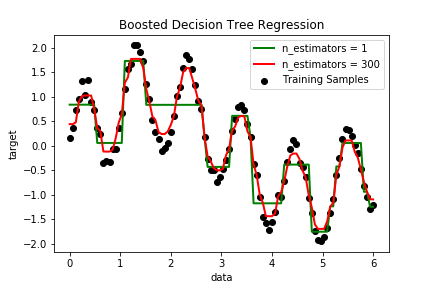
\includegraphics[width=7cm]{AdaBoost.png}
		%\caption{fig1}
	}
	\quad
	\subfigure[Bagging]{
		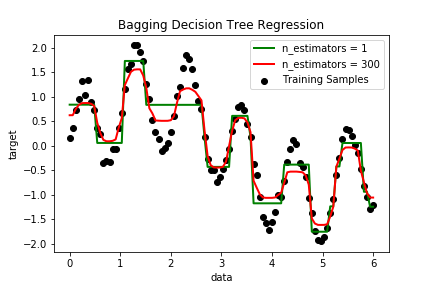
\includegraphics[width=7cm]{Bagging.png}
	}
	\caption{Try}
\end{figure}
\newpage
\section{python实现}
由于本次上机中使用了包,大可把其作为黑箱,其中具体实现细节不必深究。以下比较AdaBoost、Bagging、MultiAdaBoost、Iterative Bagging算法在分类和回归问题中的性能。

\subsection{分类问题}
首先在官方网站的示例代码的基础上进行一个二分类任务的学习和可视化任务,从而对AdaBoost、Bagging、MultiAdaBoosting和Iterative Bagging四种算法有一些基本的了解

分别运行四种算法得到:
\begin{itemize}
	\item
	AdaBoost 算法耗时0.06894421577453613 s
	\item
	Bagging 算法耗时0.01584601402282715 s
	\item
	MultiAdaBoosting算法耗时0.6348793506622314 s
	\item
	Iter Bagging算法耗时3.324193239212036 s
\end{itemize}

其得到的分类边界图分别为
\begin{figure}[htbp]
	\centering
	\subfigure[AdaBoost]{
		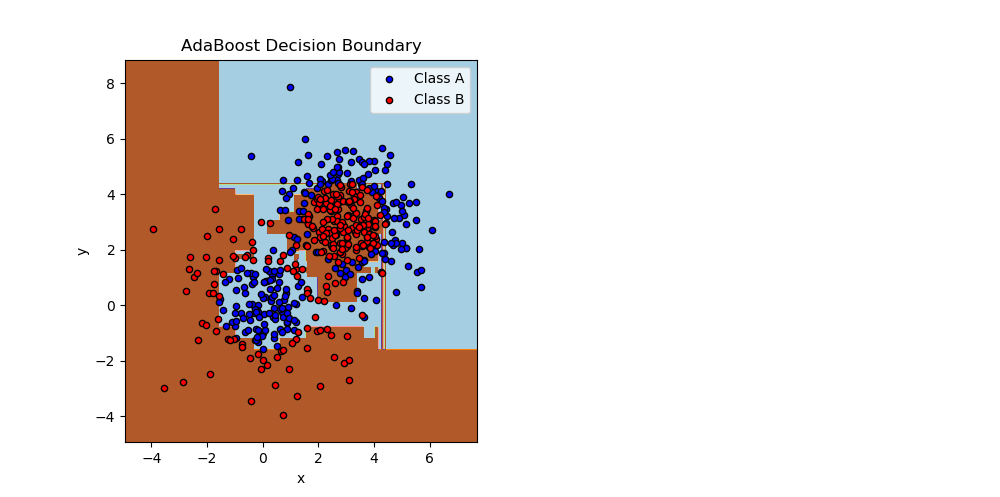
\includegraphics[width=7cm]{Ada_clf.png}
		%\caption{fig1}
	}
	\quad
	\subfigure[Bagging]{
		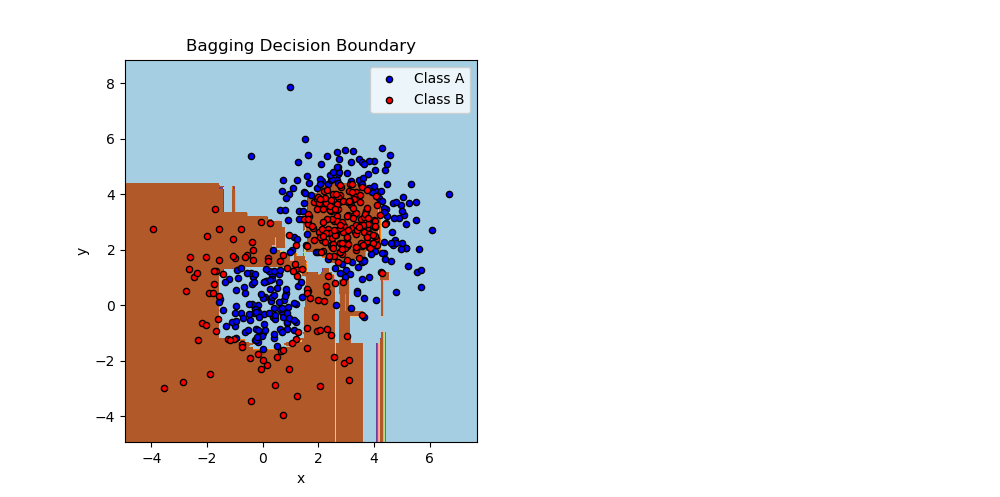
\includegraphics[width=7cm]{Bag_clf.png}
	}
	\quad
	\subfigure[Iterative Bagging]{
		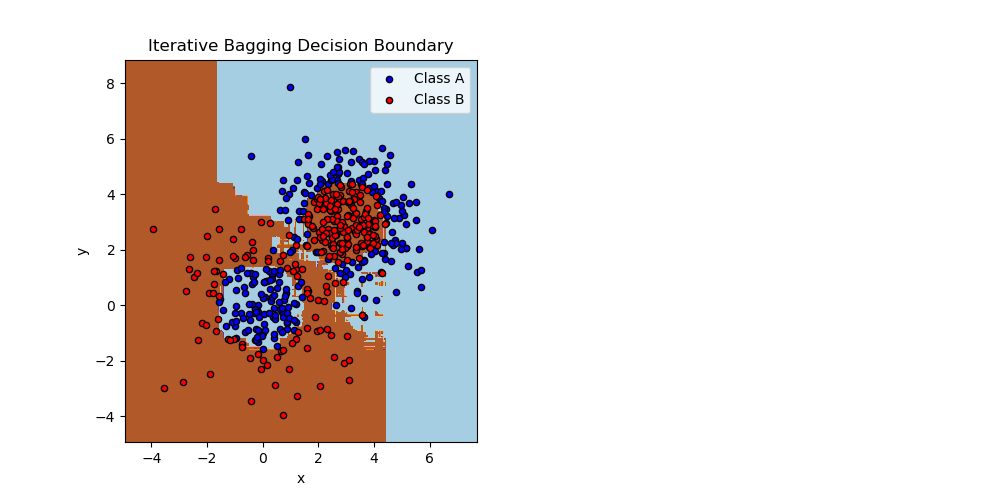
\includegraphics[width=7cm]{Iter_clf.png}
	}
	\quad
	\subfigure[MultiAdaBoost]{
		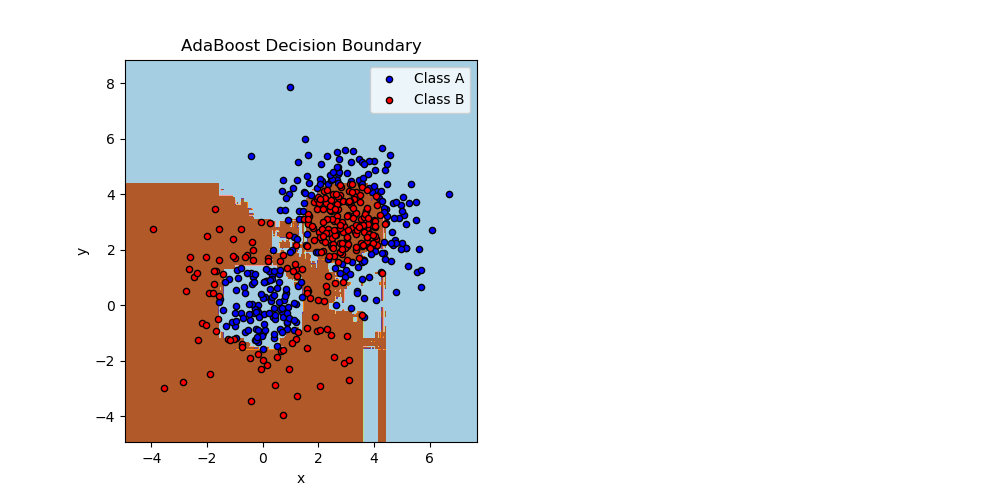
\includegraphics[width=7cm]{AdaBoost_clf.png}
	}
	\caption{Classification\_Try}
\end{figure}
综合以上信息能够得到一些简单的结果——四种算法中 AdaBoost算法得到的模型预测效果稍差(在(a)图中可以看出,在A、B两类混合的区域中分类效果较差),并且IterBagging 算法的运行时间显著长于其他三种。

\subsubsection{Breast Cancer数据集}
接下来,对于一个实际的数据集——Breast\_Cancer数据集,进行分类问题的训练,并且通过10折验证来得到习得模型的性能的度量。

首先给出算法的核心代码:
\begin{lstlisting}[language=python]
X = load_breast_cancer().data
y = load_breast_cancer().target
bdt = AdaBoostClassifier(BaggingClassifier(), n_estimators = 200)
#bdt = AdaBoostClassifier()
#bdt = BaggingClassifier()
#bdt = BaggingClassifier(AdaBoostClassifier(), 
#        max_samples = 0.63, max_features = 0.63)
bdt.fit(X, y)
\end{lstlisting}

分别运行四种算法得到运行结果

\begin{figure}[htb]
	\centering
	\includegraphics[scale=0.3]{C:/Users/linxi/AppData/Roaming/Typora/typora-user-images/1559064164043.png}
	\caption{AdaBoost}
\end{figure}

\begin{figure}[htb]
	\centering
	\includegraphics[scale=0.3]{C:/Users/linxi/AppData/Roaming/Typora/typora-user-images/1559064196197.png}
	\caption{Bagging}
\end{figure}

\begin{figure}[htb]
	\centering
	\includegraphics[scale=0.3]{C:/Users/linxi/AppData/Roaming/Typora/typora-user-images/1559064287921.png}
	\caption{MultiAdaBoosting}
\end{figure}

\begin{figure}[htb]
	\centering
	\includegraphics[scale=0.3]{C:/Users/linxi/AppData/Roaming/Typora/typora-user-images/1559064887776.png}
	\caption{Iter Bagging}
\end{figure}
\newpage
\subsubsection{wine数据集}
类似的,我们使用wine数据集,再对四种算法进行测试。有些需要注意的地方

Iterative Bagging

\begin{figure}[htb]
	\centering
	\includegraphics[scale=0.3]{C:/Users/linxi/AppData/Roaming/Typora/typora-user-images/1559115249973.png}
	\caption{Iterative Bagging}
\end{figure}

MultiBoosting

\begin{figure}[htb]
	\centering
	\includegraphics[scale=0.3]{C:/Users/linxi/AppData/Roaming/Typora/typora-user-images/1559115357326.png}
	\caption{MultiBoosting}
\end{figure}

AdaBoosting
\begin{figure}[htb]
	\centering
	\includegraphics[scale=0.3]{C:/Users/linxi/AppData/Roaming/Typora/typora-user-images/1559115398760.png}
	\caption{AdaBoosting}
\end{figure}

Bagging

\begin{figure}[htb]
	\centering
	\includegraphics[scale=0.3]{C:/Users/linxi/AppData/Roaming/Typora/typora-user-images/1559115425323.png}
	\caption{Bagging}
\end{figure}

首先,共同的结果是,Iterative Bagging算法的运行时长显著长于其他三种算法,稍有不同的情况在于,在算法的平均泛化性能方面,Bagging算法此时表现最差。因此可以初步得到,Iterative Bagging 和 MultiAdaBoost这两个算法的性能稳定地好于原本的算法。在运行所需时间的方面,Iterative Bagging算法所需时间显著多于其他三个算法。

\newpage
\subsection{回归问题}
\subsubsection{Boston数据集}
我们首先使用Boston房价数据集对四种算法在回归问题中的表现进行一些测试。
依次展示 AdaBoost、Bagging、MultiAdaBoosting、Iterative Bagging的运行结果
\begin{figure}[htb]
	\centering
	\includegraphics[scale=0.5]{C:/Users/linxi/AppData/Roaming/Typora/typora-user-images/1559111549233.png}
	\caption{AdaBoost}
\end{figure}

\begin{figure}[htb]
	\centering
	\includegraphics[scale=0.5]{C:/Users/linxi/AppData/Roaming/Typora/typora-user-images/1559111623025.png}
	\caption{Bagging}
\end{figure}

\begin{figure}[htb]
	\centering
	\includegraphics[scale=0.5]{C:/Users/linxi/AppData/Roaming/Typora/typora-user-images/1559114602851.png}
	\caption{MultiAda}
\end{figure}

\begin{figure}[htb]
	\centering
	\includegraphics[scale=0.5]{C:/Users/linxi/AppData/Roaming/Typora/typora-user-images/1559114001782.png}
	\caption{Iterative Bagging}
\end{figure}

\newpage
\subsubsection{Diabetes数据集}

再尝试一下Diabetes数据集

展示的运行结果分别是MultiBoosting、Iterative Bagging、Bagging、AdaBoosting

\begin{figure}[htb]
	\centering
	\includegraphics[scale=0.5]{C:/Users/linxi/AppData/Roaming/Typora/typora-user-images/1559116491846.png}
	\caption{MultiBoosting}
\end{figure}

\begin{figure}[htb]
	\centering
	\includegraphics[scale=0.5]{C:/Users/linxi/AppData/Roaming/Typora/typora-user-images/1559116565202.png}
	\caption{Iterative Bagging}
\end{figure}

\begin{figure}[htb]
	\centering
	\includegraphics[scale=0.5]{C:/Users/linxi/AppData/Roaming/Typora/typora-user-images/1559116603792.png}
	\caption{Bagging}
\end{figure}

\begin{figure}[htb]
	\centering
	\includegraphics[scale=0.5]{C:/Users/linxi/AppData/Roaming/Typora/typora-user-images/1559116654485.png}
	\caption{AdaBoosting}
\end{figure}

\newpage
\section{总结和思考}


\end{document}
